%--------------------
% Packages
% -------------------
\documentclass[11pt,english]{article}
\usepackage{amsfonts}
\usepackage[left=2.5cm,top=2cm,right=2.5cm,bottom=3cm,bindingoffset=0cm]{geometry}
\usepackage{amsmath, amsthm, amssymb}
\usepackage{tikz}
\usetikzlibrary{calc}
\usetikzlibrary{decorations.pathreplacing,calligraphy}
\usepackage{fancyhdr}
%\usepackage{currfile}
\usepackage{nicefrac}
\usepackage{cite}
\usepackage{graphicx}
\usepackage{caption}
\usepackage{longtable}
\usepackage{rotating}
\usepackage{lscape}
\usepackage{booktabs}
\usepackage{float}
\usepackage{placeins}
\usepackage{setspace}
\usepackage[font=itshape]{quoting}
\onehalfspacing
\usepackage{mathrsfs}
\usepackage{tcolorbox}
\usepackage{xcolor}
\usepackage{subcaption}
\usepackage{float}
\usepackage[multiple]{footmisc}
\usepackage[T1]{fontenc}
\usepackage[sc]{mathpazo}
\usepackage{listings}
\usepackage{longtable}
\definecolor{cmured}{RGB}{175,30,45}
\definecolor{macroblue}{RGB}{56,108,176}
\usepackage[format=plain,
            labelfont=bf,
            textfont=]{caption}
\usepackage[colorlinks=true,citecolor=macroblue,linkcolor=macroblue,urlcolor=macroblue]{hyperref}
\usepackage{varioref}
\usepackage{chngcntr}
\usepackage{datetime}

\definecolor{darkgreen}{RGB}{30,175,88}
\definecolor{darkblue}{RGB}{30,118,175}
\definecolor{maroon}{rgb}{0.66,0,0}
\definecolor{darkgreen}{rgb}{0,0.69,0}

%Counters
\newtheorem{theorem}{Theorem}[section] 
\newtheorem{proposition}{Proposition}
\newtheorem{lemma}{Lemma}
\newtheorem{corollary}{Corollary}
\newtheorem{assumption}{Assumption}
\newtheorem{axiom}{Axiom}
\newtheorem{case}{Case}
\newtheorem{claim}{Claim}
\newtheorem{condition}{Condition}
\newtheorem{definition}{Definition}
\newtheorem{example}{Example}
\newtheorem{notation}{Notation}
\newtheorem{remark}{Remark}


\hypersetup{ 	
pdfsubject = {},
pdftitle = {TidyTuesday Week 45},
pdfauthor = {Pranay Gundam},
linkcolor= macroblue
}


\title{\textbf{TidyTuesday Week 45}}
\author{Pranay Gundam}


%-----------------------
% Begin document
%-----------------------
\begin{document}

\maketitle

\tableofcontents

\section{Weekly Summary}


\section{Date: 2024-11-04}
\noindent \textbf{Series ID: DTBOVXDFBANM} 

\noindent This series is titled Business Motor Vehicle Loans and Leases Owned by Finance Companies, Flow and has a frequency of Monthly. The units are Millions of Dollars, Monthly Rate and the seasonal adjustment is Not Seasonally Adjusted.The observation start date is 1980-07-01 and the observation end date is 2024-08-01.The popularity of this series is 1. \\ 

\noindent \textbf{Series ID: ASHMA} 

\noindent This series is titled All Sectors; One-to-Four-Family Residential Mortgages; Asset, Level and has a frequency of Quarterly. The units are Millions of Dollars and the seasonal adjustment is Not Seasonally Adjusted.The observation start date is 1945-10-01 and the observation end date is 2024-04-01.The popularity of this series is 31. \\ 

\subsection{Regression Tables and Plots}
\begin{center}
\begin{tabular}{lclc}
\toprule
\textbf{Dep. Variable:}            & value\_fred\_ASHMA & \textbf{  R-squared:         } &     0.078   \\
\textbf{Model:}                    &        OLS         & \textbf{  Adj. R-squared:    } &     0.073   \\
\textbf{Method:}                   &   Least Squares    & \textbf{  F-statistic:       } &     14.80   \\
\textbf{Date:}                     &  Mon, 04 Nov 2024  & \textbf{  Prob (F-statistic):} &  0.000168   \\
\textbf{Time:}                     &      10:31:34      & \textbf{  Log-Likelihood:    } &   -2925.3   \\
\textbf{No. Observations:}         &          176       & \textbf{  AIC:               } &     5855.   \\
\textbf{Df Residuals:}             &          174       & \textbf{  BIC:               } &     5861.   \\
\textbf{Df Model:}                 &            1       & \textbf{                     } &             \\
\textbf{Covariance Type:}          &     nonrobust      & \textbf{                     } &             \\
\bottomrule
\end{tabular}
\begin{tabular}{lcccccc}
                                   & \textbf{coef} & \textbf{std err} & \textbf{t} & \textbf{P$> |$t$|$} & \textbf{[0.025} & \textbf{0.975]}  \\
\midrule
\textbf{const}                     &    6.187e+06  &     3.28e+05     &    18.857  &         0.000        &     5.54e+06    &     6.83e+06     \\
\textbf{value\_fred\_DTBOVXDFBANM} &    -365.5684  &       95.034     &    -3.847  &         0.000        &     -553.137    &     -178.000     \\
\bottomrule
\end{tabular}
\begin{tabular}{lclc}
\textbf{Omnibus:}       & 378.495 & \textbf{  Durbin-Watson:     } &    0.212  \\
\textbf{Prob(Omnibus):} &   0.000 & \textbf{  Jarque-Bera (JB):  } &   15.348  \\
\textbf{Skew:}          &   0.157 & \textbf{  Prob(JB):          } & 0.000465  \\
\textbf{Kurtosis:}      &   1.588 & \textbf{  Cond. No.          } & 3.73e+03  \\
\bottomrule
\end{tabular}
%\caption{OLS Regression Results}
\end{center}

Notes: \newline
 [1] Standard Errors assume that the covariance matrix of the errors is correctly specified. \newline
 [2] The condition number is large, 3.73e+03. This might indicate that there are \newline
 strong multicollinearity or other numerical problems.

\begin{figure}
\centering
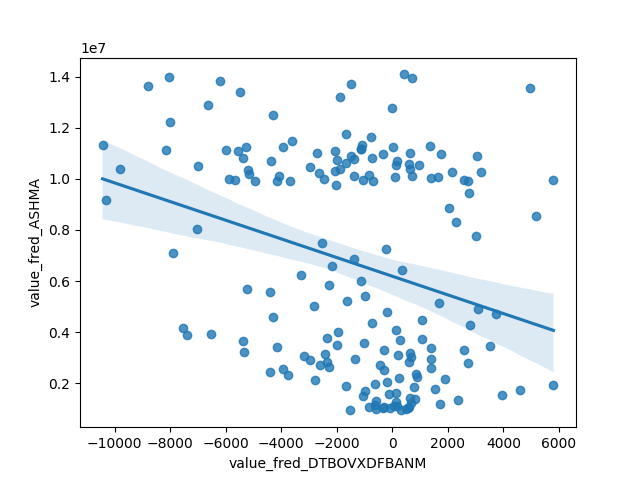
\includegraphics[scale = 0.9]{plots/plot_2024-11-04.png}
\caption{Regression Plot for 2024-11-04}
\end{figure}
\newpage

\section{Date: 2024-11-05}
\noindent \textbf{Series ID: CES6055000001} 

\noindent This series is titled All Employees, Management of Companies and Enterprises and has a frequency of Monthly. The units are Thousands of Persons and the seasonal adjustment is Seasonally Adjusted.The observation start date is 1990-01-01 and the observation end date is 2024-10-01.The popularity of this series is 3. \\ 

\noindent \textbf{Series ID: PCU443141443141} 

\noindent This series is titled Producer Price Index by Industry: Household Appliance Stores and has a frequency of Monthly. The units are Index Jun 2003=100 and the seasonal adjustment is Not Seasonally Adjusted.The observation start date is 2003-06-01 and the observation end date is 2019-05-01.The popularity of this series is 1. \\ 

\subsection{Regression Tables and Plots}
\begin{center}
\begin{tabular}{lclc}
\toprule
\textbf{Dep. Variable:}             & value\_fred\_PCU443141443141 & \textbf{  R-squared:         } &     0.004   \\
\textbf{Model:}                     &             OLS              & \textbf{  Adj. R-squared:    } &    -0.001   \\
\textbf{Method:}                    &        Least Squares         & \textbf{  F-statistic:       } &    0.7508   \\
\textbf{Date:}                      &       Tue, 05 Nov 2024       & \textbf{  Prob (F-statistic):} &    0.387    \\
\textbf{Time:}                      &           15:24:09           & \textbf{  Log-Likelihood:    } &   -722.87   \\
\textbf{No. Observations:}          &               192            & \textbf{  AIC:               } &     1450.   \\
\textbf{Df Residuals:}              &               190            & \textbf{  BIC:               } &     1456.   \\
\textbf{Df Model:}                  &                 1            & \textbf{                     } &             \\
\textbf{Covariance Type:}           &          nonrobust           & \textbf{                     } &             \\
\bottomrule
\end{tabular}
\begin{tabular}{lcccccc}
                                    & \textbf{coef} & \textbf{std err} & \textbf{t} & \textbf{P$> |$t$|$} & \textbf{[0.025} & \textbf{0.975]}  \\
\midrule
\textbf{const}                      &      97.0263  &        7.022     &    13.817  &         0.000        &       83.175    &      110.878     \\
\textbf{value\_fred\_CES6055000001} &      -0.0029  &        0.003     &    -0.867  &         0.387        &       -0.010    &        0.004     \\
\bottomrule
\end{tabular}
\begin{tabular}{lclc}
\textbf{Omnibus:}       & 63.169 & \textbf{  Durbin-Watson:     } &    0.041  \\
\textbf{Prob(Omnibus):} &  0.000 & \textbf{  Jarque-Bera (JB):  } &   10.571  \\
\textbf{Skew:}          &  0.077 & \textbf{  Prob(JB):          } &  0.00507  \\
\textbf{Kurtosis:}      &  1.861 & \textbf{  Cond. No.          } & 1.92e+04  \\
\bottomrule
\end{tabular}
%\caption{OLS Regression Results}
\end{center}

Notes: \newline
 [1] Standard Errors assume that the covariance matrix of the errors is correctly specified. \newline
 [2] The condition number is large, 1.92e+04. This might indicate that there are \newline
 strong multicollinearity or other numerical problems.

\begin{figure}
\centering
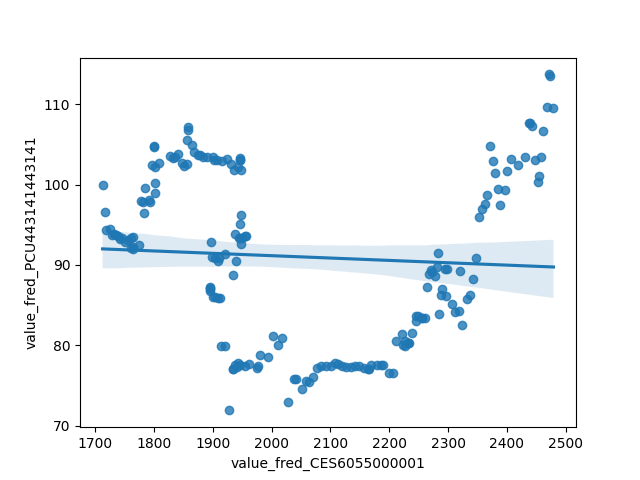
\includegraphics[scale = 0.9]{plots/plot_2024-11-05.png}
\caption{Regression Plot for 2024-11-05}
\end{figure}
\newpage

\include{tex_things/day_2024-11-06}
\include{tex_things/day_2024-11-07}
\include{tex_things/day_2024-11-08}
\include{tex_things/day_2024-11-09}
\include{tex_things/day_2024-11-10}

\end{document}
